%!TEX program = xelatex
\documentclass[a4paper,UTF8]{ctexart}
\usepackage[unicode=true,colorlinks,urlcolor=blue,linkcolor=blue,bookmarksnumbered=true]{hyperref}
\usepackage{latexsym,amssymb,amsmath,amsbsy,amsopn,amstext,amsthm,amsxtra,color,multicol,bm,calc,ifpdf}
\usepackage{graphicx}
\usepackage{diagbox}   % 绘制表格斜线
\usepackage{enumerate}
\usepackage{epstopdf}
\usepackage{fancyhdr}
\usepackage{subfigure}
\usepackage{listings}
\usepackage{multirow}
\usepackage{makeidx}
\usepackage{xcolor} 
\usepackage{fontspec}                            % 建立索引宏包
\graphicspath{{figures/}}  % 设置图片搜索路径
\theoremstyle{plain} \newtheorem{theorem}{定理}[section]
\theoremstyle{plain} \newtheorem{definition}{定义}[section]
\theoremstyle{plain} \newtheorem{lemma}{引理}[section]
\theoremstyle{plain} \newtheorem{proposition}{命题}[section]
\theoremstyle{plain} \newtheorem{example}{例}[section]
\theoremstyle{plain} \newtheorem{remark}{注}[section]
\theoremstyle{plain} \newtheorem{corollary}{推论}[section]
\newfontfamily\courier{Courier New}
\lstset{linewidth=1.1\textwidth,
        numbers=left, %设置行号位置 
        basicstyle=\small\courier,
        numberstyle=\tiny\courier, %设置行号大小  
        keywordstyle=\color{blue}\courier, %设置关键字颜色  
        %identifierstyle=\bf,
        commentstyle=\it\color[cmyk]{1,0,1,0}\courier, %设置注释颜色 
        stringstyle=\it\color[RGB]{128,0,0}\courier,
        %framexleftmargin=10mm,
        frame=single, %设置边框格式  
        backgroundcolor=\color[RGB]{245,245,244},
        %escapeinside=``, %逃逸字符(1左面的键),用于显示中文  
        breaklines, %自动折行  
        extendedchars=false, %解决代码跨页时,章节标题,页眉等汉字不显示的问题  
        xleftmargin=2em,xrightmargin=2em, aboveskip=1em, %设置边距  
        tabsize=4, %设置tab空格数  
        showspaces=false %不显示空格  
        basicstyle=\small\courier
       }  
\newenvironment{mysolution}{{\color{blue} 解}: }{{\color{magenta}\qed}}
\newcommand\diff{\,{\mathrm d}} %定义微分d
\newcommand{\p}[3]{\frac{\partial^{#1}#2}{\partial{#3}^{#1}}}  %定义求偏导算子
\newcommand{\ucite}[1]{\textsuperscript{\cite{#1}}}  %参考文献引用:上标用\ucite{ },文中用\cite{ }

\begin{document}
\title{

\includegraphics[width=0.65\textwidth]{onepiece.pdf}\\
\vspace{2em}
\textbf{朴素贝叶斯学习笔记}}
\author{\emph{李向阳} \quad {\color{blue} d1142845997@gmail.com} }
\date{}


\maketitle
\thispagestyle{empty}

\newpage


\tableofcontents

\newpage

\section{引入}
目前为止, 我们介绍的大多数模型(线性回归、Logistic 回归、SVM、神经网络等)均被称为“判别模型”(Discriminative Learning Algorithm), 本次介绍的朴素贝叶斯模型属于“生成模型”(Generative
Learning Algorithm). 关于判别模型与生成模型的对比, 可以参考相关资料, 这里以分类问题为例稍微解释一下.

在 Logistic 回归模型中, 我们是对什么建模呢? 其实我们是对概率(分布)$p(y | \bm{x}; \bm{\theta})$进行的建模, 即给定样本$\bm{x}$后类别$y$的条件分布. 在那里, 我们假设$p(y | \bm{x}; \bm{\theta}) = h_{\bm{\theta}}(\bm{x}) = \sigma(\bm{\theta}^{T} \bm{x})$. 也就是说, 直接对后验概率(简记为$p(y | \bm{x})$)建模. 这种模型就称为判别模型.

而所谓生成模型, 实际上是对$p(\bm{x} | y)$进行建模, 然后利用 Bayes 公式(\ref{bayeseq}))间接算出后验概率$p(y | \bm{x})$, 然后再进行判断.
\begin{equation}\label{bayeseq}
p(y | \bm{x}) = \frac{p(\bm{x}, y)}{p(\bm{x})} = \frac{p(\bm{x} | y) \cdot p(y)}{p(\bm{x})}
\end{equation}

其中$p(y)$是先验概率. 在分类问题中, 我们将样本归为后验概率最大的那一类, 即
\begin{align*}
\arg \max_{y} p(y | \bm{x}) & = \arg \max_{y} \frac{p(\bm{x} | y) p(y)}{p(\bm{x})} \\ 
& = \arg \max_{y} p(\bm{x} | y) p(y)
\end{align*}

注意到$p(\bm{x} | y)$是所有属性上的联合概率, 难以从有限的训练样本直接估计而得. 为了避开这个障碍, 朴素贝叶斯分类器(Naive Bayes Classifier)采用了“属性条件独立性假设”, 即假设样本的$n$个属性独立的对分类结果发生影响, 也就是
\begin{equation*}
p(\bm{x} | y) = \prod_{i=1}^{n} p(x_{i} | y)
\end{equation*}

“朴素”的含义即由此而来. 下面就来介绍朴素贝叶斯模型, 这里先稍微提一下, 我们主要假设样本的属性取值是离散的, 如果有连续的部分当然也有办法处理. 此外, 如果$n$个属性的取值均为连续的, 那么我们可能更倾向于高斯判别模型, 这个下面也会提到.


\section{基本模型}
为了与之前的记号保持一致, 设样本$\bm{x}$有$n$个特征, $\bm{x} = (x_1, x_2, \cdots, x_n)$, 对应的类标记设为$y$, 不妨设有$K$个类, 用$y = c_{k}$表示样本属于第$k$类, 即$y \in \{c_1, c_2, \cdots, c_K\}$. 我们假设有$m$个样本, $(\bm{x}^{(i)}, y^{(i)}), i = 1, 2, \cdots, m$. 
\begin{equation*}
\bm{x}^{(i)} = (x_{1}^{(i)}, x_{2}^{(i)}, \cdots, x_{n}^{(i)})^{T}
\end{equation*}


对于给定样本$\bm{x}$, 我们将其归为后验概率最大的那一类, 即
\begin{equation*}
y = \max_{c_k} p(y = c_k | \bm{x})
\end{equation*}

我们知道
\begin{equation*}
p(y = c_k | \bm{x}) = \frac{p(y = c_k) p(\bm{x} | y = c_k)}{p(\bm{x})}
\end{equation*}

因此分类规则为
\begin{align*}
y & = \max_{c_k} p(y = c_k) p(\bm{x} | y = c_k) \\ 
& = \max_{c_k} p(y = c_k) \prod_{i=1}^{n} p(x_i | y = c_k)
\end{align*}

其中$p(x_i | y = c_k)$表示该样本属于第$k$类的基础上, 其第$i$个属性取值为$x_i$的条件概率(本文有时用$x_i$表示第$i$个属性对应的变量, 有时表示样本$\bm{x}$在第$i$个属性上的取值, 联系上下文注意含义即可).

于是, 我们需要的估计的参数有类的先验概率$p(y = c_{k}), k=1,2,\cdots,K$, 这个很容易估计, 假设所有的训练样本集即为$D$, 令$D_{k}$表示训练样本中第$k$类样本组成的集合, 则先验概率的一个合理的估计就是
\begin{equation}\label{pioreq1}
p(y = c_k) = \frac{|D_k|}{|D|}
\end{equation}

事实上, 不难证明, 先验概率的极大似然估计正是
\begin{equation}\label{pioreq2}
p(y = c_k) = \frac{1}{m} \sum_{i=1}^{m} \mathbb{I}(y^{(i)} = c_k)
\end{equation}

其中$\mathbb{I}(\cdot)$是示性函数. 式(\ref{pioreq1})与式(\ref{pioreq2})是完全一样的.

另外需要估计的参数是$p(x_i | y = c_k)$. 令$D_{k, x_i}$表示$D_{k}$中在第$i$个属性上取值为$x_i$的样本组成的集合, 则条件概率另外需要估计的参数是$p(x_i | y = c_k)$的一个合理的估计为
\begin{equation}\label{condeq1}
p(x_i | y = c_k) = \frac{|D_{k, x_i}|}{|D_k|}
\end{equation}

事实上, 设第$j$个特征$x_j$可能的取值集合为$\{a_{j1}, a_{j2}, \cdots, a_{j s_j}\}$, 则条件概率$p(a_{jl} | y = c_k)$的极大似然估计是
\begin{equation}\label{condeq2}
\begin{split}
& p(a_{jl} | y = c_k) = \frac{\sum_{i=1}^{m} \mathbb{I}(x_{j}^{(i)} = a_{jl}, y^{(i)} = c_k)}{\sum_{i=1}^{m} \mathbb{I}(y^{(i)} = c_k)} \\ 
& j = 1,2,\cdots,n; \quad l = 1,2,\cdots,s_{j}; \quad k=1,2,\cdots,K
\end{split}
\end{equation}

式(\ref{condeq1})与式(\ref{condeq2})表达的含义也是一样的.

估计出所有的参数以后, 对于一个新的样本$\bm{x}^{(0)} = (x_{1}^{(0)}, x_{2}^{(0)}, \cdots, x_{n}^{(0)})^{T}$, 计算下式即可判断其类别
\begin{align*}
y^{(0)} & = \max_{c_k} p(y = c_k) p(\bm{x}^{(0)} | y = c_k) \\ 
& = \max_{c_k} p(y = c_k) \prod_{i=1}^{n} p(x_{i}^{(0)} | y = c_k)
\end{align*}

下面举一个例子, 来自李航的《统计学习方法》.

\begin{example}
下表\ref{examp1}是一个训练样本集$D$, 包含$15$个样本, 其中$x_1, x_2$为样本的特征, 容易看出, 其取值的集合分别为$A_{1} = \{1, 2, 3\}, A_{2} = \{S, M, L\}$, $y$为类标记, $y \in \{-1, 1\}$. 我们要用这些训练样本学习出一个朴素贝叶斯分类器. 并且, 假设有一个新样本$\bm{x}^{(0)} = (2, S)^{T}$, 我们要判断它的类别.

\begin{table}[!htb]
\centering
\caption{训练样本集}
\label{examp1}
\begin{tabular}{cccc}
	\hline
    % after \: \hline or \cline{col1-col2} \cline{col3-col4} ...
    \textbf{ID} & \textbf{$x_1$} & \textbf{$x_2$} & \textbf{$y$} \\
    \hline
    1   &  1  &  S  &  -1 \\
    \hline
    2   &  1  &  M  &  -1 \\
    \hline
    3   &  1  &  M  &  1 \\
    \hline
    4   &  1  &  S  &  1 \\
    \hline
    5   &  1  &  S  &  -1 \\
    \hline
    6   &  2  &  S  &  -1 \\
    \hline
    7   &  2  &  M  &  -1 \\
    \hline
    8   &  2  &  M  &  1 \\
    \hline
    9   &  2  &  L  &  1 \\
    \hline
    10   &  2  &  L  &  1 \\
    \hline
    11   &  3  &  L  &  1 \\
    \hline
    12   &  3  &  M  &  1 \\
    \hline
    13   &  3  &  M  &  1 \\
    \hline
    14   &  3  &  L  &  1 \\
    \hline
    15   &  3  &  L  &  -1 \\
    \hline
\end{tabular}
\end{table}

\end{example}

\begin{mysolution}
首先, 估计类别的先验概率, 正类集合设为$D_1(y = 1)$, 包含$9$个样本, 负类集合设为$D_2(y = -1)$, 包含$6$个样本, 因此
\begin{equation*}
p(y = 1) = \frac{9}{15}, p(y = -1) = \frac{6}{15} 
\end{equation*}

在估计条件概率, 也很容易, 比如先把正类集合拿出来, 为了方便, 列出如下表\ref{examp1-posit}.
\begin{table}[!htb]
\centering
\caption{训练样本集中的正类}
\label{examp1-posit}
\begin{tabular}{cccc}
	\hline
    % after \: \hline or \cline{col1-col2} \cline{col3-col4} ...
    \textbf{ID} & \textbf{$x_1$} & \textbf{$x_2$} & \textbf{$y$} \\
    \hline
    3   &  1  &  M  &  1 \\
    \hline
    4   &  1  &  S  &  1 \\
    \hline
    8   &  2  &  M  &  1 \\
    \hline
    9   &  2  &  L  &  1 \\
    \hline
    10   &  2  &  L  &  1 \\
    \hline
    11   &  3  &  L  &  1 \\
    \hline
    12   &  3  &  M  &  1 \\
    \hline
    13   &  3  &  M  &  1 \\
    \hline
    14   &  3  &  L  &  1 \\
    \hline
\end{tabular}
\end{table}

由此很容易算得
\begin{align*}
p(x_1 = 1 | y = 1) = \frac{2}{9}, \quad p(x_1 = 2 | y = 1) = \frac{3}{9}, \quad p(x_1 = 3 | y = 1) = \frac{4}{9} \\ 
p(x_2 = S | y = 1) = \frac{1}{9}, \quad p(x_2 = M | y = 1) = \frac{4}{9}, \quad p(x_1 = 3 | y = 1) = \frac{4}{9}
\end{align*}

同理, 可列出负类的表格, 计算条件概率如下
\begin{align*}
p(x_1 = 1 | y = -1) = \frac{3}{6}, \quad p(x_1 = 2 | y = -1) = \frac{2}{6}, \quad p(x_1 = 3 | y = -1) = \frac{1}{6} \\ 
p(x_2 = S | y = -1) = \frac{3}{6}, \quad p(x_2 = M | y = -1) = \frac{2}{6}, \quad p(x_2 = L | y = -1) = \frac{1}{6}
\end{align*}

这样所有的参数就估计出来了.

对于新样本$\bm{x}^{(0)} = (2, S)^{T}$, 做计算
\begin{align*}
p(y = 1) \prod_{i=1}^{2} p(x_{i}^{(0)} | y = 1) & = p(y = 1) \cdot p(x_1 = 2 | y = 1) p(x_2  = S | y = 1) \\ 
& = \frac{9}{15} \cdot \frac{3}{9} \cdot \frac{1}{9} = \frac{1}{45}
\end{align*}

同理可得
\begin{align*}
p(y = -1) \prod_{i=1}^{2} p(x_{i}^{(0)} | y = -1) & = p(y = -1) \cdot p(x_1 = 2 | y = -1) p(x_2  = S | y = -1) \\ 
& = \frac{6}{15} \cdot \frac{2}{6} \cdot \frac{3}{6} = \frac{1}{15}
\end{align*}

显然后者比较大, 所以$y^{(0)} = -1$, 即把新样本归为负类.

\end{mysolution}


\section{连续属性与 Laplace 平滑}
\subsection{连续属性}
在上面的讨论和例子中, 假设属性的取值是离散的, 若有连续属性, 一般假设连续属性服从高斯分布, 即$p(x_i | y = c_k) \sim \mathcal{N}(\mu_{k,i}, \sigma_{k,i}^2)$, 其中$\mu_{k,i}$和$\sigma_{k,i}^2$分别是第$k$类样本在第$i$个属性上取值的均值和方差(计算时由样本估计), 进而可得条件概率的估计
\begin{equation*}
p(x_i | y = c_k) = \frac{1}{\sqrt{2 \pi} \sigma_{k,i}} \exp \left( - \frac{(x_i - \mu_{k,i})^2}{2 \sigma_{k,i}^2} \right)
\end{equation*}


下面我们举一个属性全是连续值的例子, 该例子来自维基百科, 通过测量人的一些特征, 包括身高、体重和脚长(脚的尺寸), 来判断一个人是男性还是女性. 训练样本如下表\ref{gendersample}.
\begin{table}[!htb]
\centering
\caption{男女特征样本}
\label{gendersample}
\begin{tabular}{ccccc}
	\hline
    % after \: \hline or \cline{col1-col2} \cline{col3-col4} ...
	ID & 身高(英尺) & 体重(磅) &  脚长(英寸)  & 性别 \\
	\hline 
	1 & 6 & 180 & 12 & 男 \\ 
	\hline
	2 & 5.92 & 190 & 11 & 男 \\ 
	\hline
	3 & 5.58 & 170 & 12 & 男 \\ 
	\hline
	4 & 5.92 & 165 & 10 & 男 \\ 
	\hline
	5 & 5 & 100 & 6 & 女 \\ 
	\hline
	6 & 5.5 & 150 & 8 & 女 \\ 
	\hline
	7 & 5.42 & 130 & 7 & 女 \\ 
	\hline
	8 & 5.75 & 150 & 9 & 女 \\ 
	\hline
\end{tabular}
\end{table}

现在有一个样本$\bm{x}^{(0)} = (6, 130, 8)^{T}$, 我们要判断其性别.

不妨用$x_1, x_2, x_3$表示$3$个属性, 用$y = 1$表示男性, $y = -1$表示女性, 显然, 先验概率为$p(y = 1) = p(y = -1) = \frac{1}{2}$. 为了得到条件概率的估计, 假设各个属性服从正态分布, 可得下表\ref{gender}.
\begin{table}[!htb]
\centering
\caption{男女表格}
\label{gender}\begin{tabular}{|l|l|l|l|l|l|l|}
\hline
\multirow{2}{*}{性别} & \multicolumn{2}{c|}{身高} & \multicolumn{2}{c|}{体重} & \multicolumn{2}{c|}{脚长} \\ \cline{2-7} 
                    & 均值         & 方差         & 均值          & 方差        & 均值          & 方差        \\ \hline
男                   & 5.855      & 0.035      & 176.25      & 122.92     & 11.25       & 0.92      \\ \hline
女                   & 5.418      & 0.097      & 132.50      & 558.33     & 7.50        & 1.67      \\ \hline
\end{tabular}
\end{table}

现在就可以计算条件概率
\begin{equation*}
p(x_1 = 6 | y = 1) = \frac{1}{\sqrt{2 \pi} \sigma} \exp \left( - \frac{(6 - \mu)^2}{2 \sigma^2} \right) = 1.5792
\end{equation*}

其中的$\mu = 5.855, \sigma^2 = 0.035$, 是由上表\ref{gender}获得. 同理可得
\begin{align*}
p((x_2 = 130 | y = 1)) & = 5.988 \times 10^{-6} \\ 
p((x_3 = 8 | y = 1)) & = 1.336 \times 10^{-3}
\end{align*}

于是可得
\begin{equation*}
p(y = 1) \prod_{i=1}^{3} p(x_{i}^{(0)} | y = 1) = 6.1984 \times 10^{-9}
\end{equation*}

同样计算可得
\begin{equation*}
p(y = - 1) \prod_{i=1}^{3} p(x_{i}^{(0)} | y = - 1) = 5.3788 \times 10^{-4}
\end{equation*}

所以判断新样本的$y^{(0)} = -1$, 即归为女性.


\subsection{Laplace 平滑}
用以上方法计算时, 有可能会出现概率为$0$的情况, 为什么呢?

试想一下, 若某个属性值在训练样本集中没有与某个类同时出现过, 则它的条件概率估计刚好就是$0$了.

要解决这一问题, 方法是采用贝叶斯估计来估计参数, 具体的, 条件概率的贝叶斯估计是
\begin{equation}\label{condbayes}
p_{\lambda} (a_{jl} | y = c_k) = \frac{\sum_{i=1}^{m} \mathbb{I}(x_{j}^{(i)} = a_{jl}, y^{(i)} = c_k) + \lambda}{\sum_{i=1}^{m} \mathbb{I}(y^{(i)} = c_k) + s_{j} \lambda}
\end{equation}

其中$\lambda \geqslant 0$, 这等价于在属性的各个取值的频数上赋予一个正数$\lambda > 0$. 当$\lambda = 0$时就是极大似然估计. 我们常取$\lambda = 1$, 这时称为拉普拉斯平滑(Laplace smoothing). 显然, 对任何$l = 1,2,\cdots, s_{j}, k = 1,2,\cdots,K$, 都有
\begin{align*}
p_{\lambda} (a_{jl} | y = c_k) & > 0 \\ 
\sum_{l=1}^{s_{j}} p(a_{jl} | y = c_k) & = 1
\end{align*}

这表明式(\ref{condbayes})确实是一种概率分布. 同样, 先验概率的贝叶斯估计是
\begin{equation*}
p_{\lambda} (y = c_k) = \frac{\sum_{i=1}^{m} \mathbb{I}(y = c_k) + \lambda}{m + K \lambda}
\end{equation*}

总之, 采用 Laplace 平滑的话, $K$表示训练样本集$D$可能的类别数, 用$K_i$表示第$i$个属性可能的取值数, 则参数估计为
\begin{align*}
p(y = c_k) & = \frac{|D_k| + 1}{|D| + K} \\ 
p(x_i | y = c_k) & = \frac{|D_{k,x_i}| + 1}{|D_c| + K_i}
\end{align*}




\section{关于 Naive Bayes 的补充}
\subsection{Naive Bayes 与 Bayes 判别的区别}
在数据分析方法课程中, 我们讲了判别分析, 其中有距离判别和 Bayes 判别, 距离判别下面不提, 关键是这里的朴素贝叶斯判别与我们讲过的贝叶斯判别有什么区别呢?

首先明确一点, 我们讲过的贝叶斯判别是一种生成模型, 虽然名称叫“判别”(其实就是分类的意思), 但是它是学习到了总体的特征再进行分类的, 所以属于生成模型.

实际上, 我们在数据分析方法中讲的贝叶斯判别是一个大的框架, 更多的是从贝叶斯统计的角度来进行分类. 以两个类(也就是两个总体)为例, 如果假设每个总体都服从多元高斯分布, 那么 Bayes 判别其实就是高斯判别分析, 这在 Andrew Ng 的机器学习的 Notes 中也提到了(其中还提到了高斯判别分析与 Logistic 回归的关系, 推广来说就是生成模型与判别模型的关系). 我们一开始提到说如果样本的属性都是连续值, 我们可能会倾向于高斯判别分析, 而如果有离散值就会使用朴素贝叶斯分类器, 但是在上面男女性别的例子中, 我们看到属性值也全部都是连续的, 在这种情况下, 朴素贝叶斯分类器与高斯判别分析的区别在哪呢?

仔细想一下就明白了, 在高斯判别分析中, 我们是把一个类看成一个总体, 这个总体是服从多维正态分布的, 我们知道多维正态分布的每个维度之间可不一定是独立的. 而朴素贝叶斯呢? 它是假设每个单独的维度(特征)是服从一维正态分布, 而且每个特征之间是相互独立的, 这就是它们最大的区别.


\subsection{线性判别分析}
上面提到了距离判别, 这是在数据分析方法课程中讲的, 其实就是线性判别分析(Linear Discriminant Analysis, LDA), 也称 Fisher 线性判别(Fisher Linear Discriminant). (有个 topic 模型也叫做 LDA, 不过名字叫做 Latent Dirichlet Allocation). 
特别的, 当假设总体服从多维正态分布时, 就是高斯判别分析(Gaussian Discriminant Analysis). 这是大多数材料上的一些概念, 它们之间既有联系, 也有区别.

关于 LDA, 在数据分析课上已经讲过推导, 但要注意的是, 当时是直接从距离判别的角度出发的, 然而在大多数材料中, 比如 PRML 和周志华的《机器学习》中,都是从投影角度出发的, 最小化组内方差, 最大化组间方差, 如下图 \ref{fig:lda} 所示.
\begin{figure}[!htb]
    \centering
    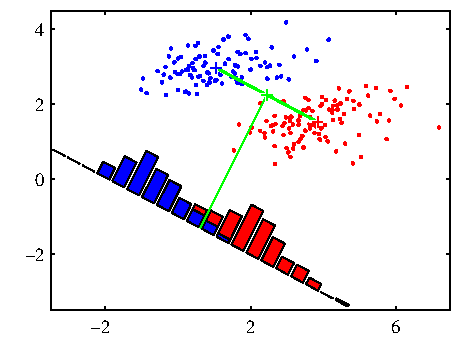
\includegraphics[width = 0.85 \textwidth]{lda-fig.pdf}
    \caption{LDA 示意图}
    \label{fig:lda}
\end{figure}

具体推导可见 PRML 或者周志华的《机器学习》, 这篇博客 \url{http://www.cnblogs.com/jerrylead/archive/2011/04/21/2024389.html} 也不错, 这里就略过了. 推导中可以用到矩阵的广义特征值和特征向量, 这可以参考张贤达的《矩阵分析与应用》一书.

最后再提一点, LDA 和 Logistic 回归都属于(广义)线性分类方法的一种, 线性分类方法还有很多, 比如将最小二乘拟合用到分类中, 这些东西也都不难, 可以参考 PRML 一书. 大多数材料比如 PRML, ESL 等都把线性模型放在了前几章, 而线性判别、Bayes 判别我已经在数据分析课上学过, 所以一直到这篇笔记为了对比才把 LDA 等补充出来.




\section{总结}
\subsection{参考资料}
\begin{enumerate}[(1)]
\item Bishop 的 PRML

\item 李航的《统计学习方法》

\item 周志华的《机器学习》

\item 维基: \url{https://en.wikipedia.org/wiki/Naive_Bayes_classifier}, 有男女的那个例子.

\item JerryLead 的博客: \url{http://www.cnblogs.com/jerrylead/archive/2011/03/05/1971903.html}, 提到了判别模型和生成模型, 实际上这篇博客是 Andrew Ng 机器学习 Notes 的英文翻译, 他的另一篇博客 \url{http://www.cnblogs.com/jerrylead/archive/2011/04/21/2024384.html} 也讲述了 LDA.
\end{enumerate}







\newpage

\section*{附录}








\end{document}